\section{RRTGoal\-Bias  Class Reference}
\label{classRRTGoalBias}\index{RRTGoalBias@{RRTGoal\-Bias}}
With some probability, choose the goal instead of a random sample. 


{\tt \#include $<$rrt.h$>$}

Inheritance diagram for RRTGoal\-Bias::\begin{figure}[H]
\begin{center}
\leavevmode
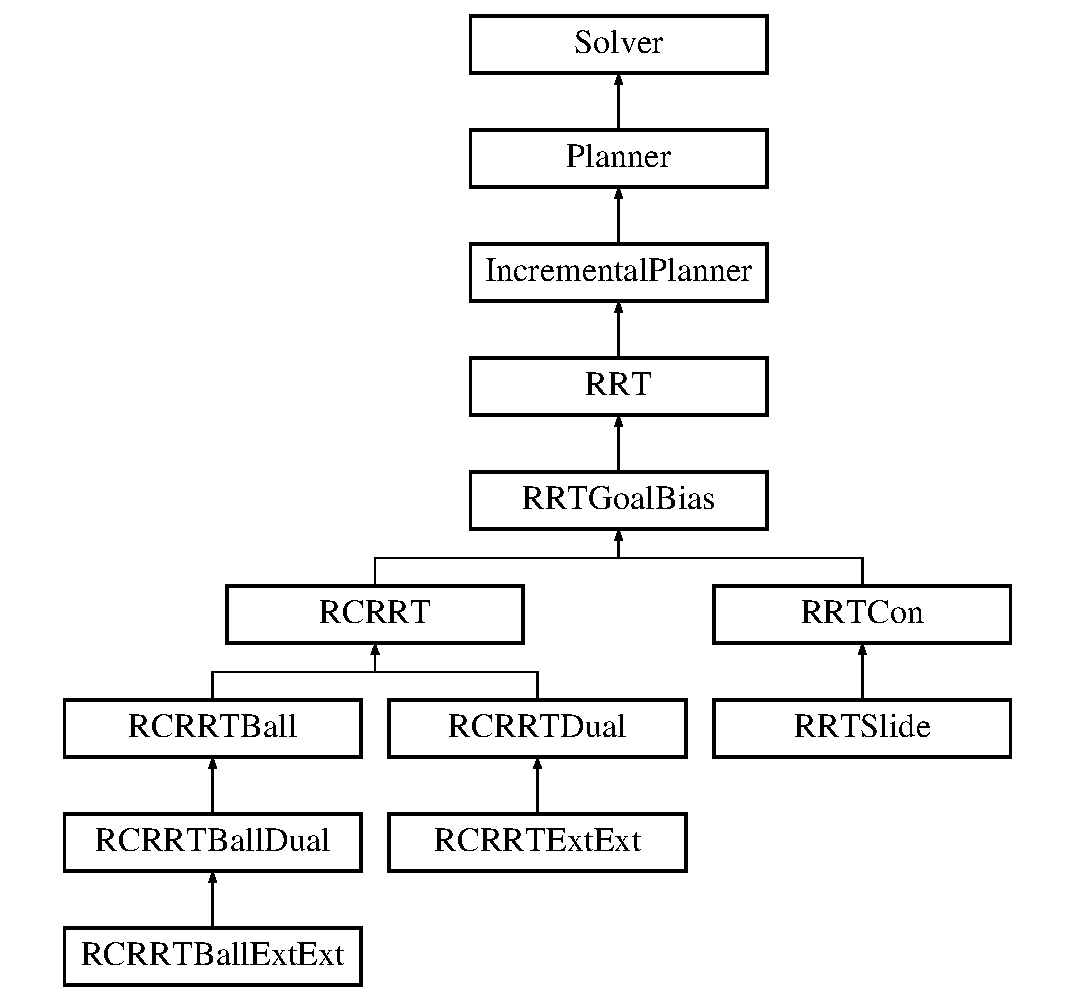
\includegraphics[height=9cm]{classRRTGoalBias}
\end{center}
\end{figure}
\subsection*{Public Methods}
\begin{CompactItemize}
\item 
{\bf RRTGoal\-Bias} ({\bf Problem} $\ast$p)
\item 
virtual {\bf $\sim$RRTGoal\-Bias} ()
\end{CompactItemize}
\subsection*{Public Attributes}
\begin{CompactItemize}
\item 
double {\bf Goal\-Prob}
\end{CompactItemize}
\subsection*{Protected Methods}
\begin{CompactItemize}
\item 
virtual {\bf MSLVector} {\bf Choose\-State} ()
\begin{CompactList}\small\item\em Pick a state using some sampling technique.\item\end{CompactList}\end{CompactItemize}


\subsection{Detailed Description}
With some probability, choose the goal instead of a random sample.

Instead of choosing a state at random, this planner chooses with probability Goal\-Prob the Goal\-State. It can be considered as a  biased coin toss in which heads yields the goal state, and tails yields a random sample. 



\subsection{Constructor \& Destructor Documentation}
\index{RRTGoalBias@{RRTGoal\-Bias}!RRTGoalBias@{RRTGoalBias}}
\index{RRTGoalBias@{RRTGoalBias}!RRTGoalBias@{RRTGoal\-Bias}}
\subsubsection{\setlength{\rightskip}{0pt plus 5cm}RRTGoal\-Bias::RRTGoal\-Bias ({\bf Problem} $\ast$ {\em p})}\label{classRRTGoalBias_a0}


\index{RRTGoalBias@{RRTGoal\-Bias}!~RRTGoalBias@{$\sim$RRTGoalBias}}
\index{~RRTGoalBias@{$\sim$RRTGoalBias}!RRTGoalBias@{RRTGoal\-Bias}}
\subsubsection{\setlength{\rightskip}{0pt plus 5cm}virtual RRTGoal\-Bias::$\sim$RRTGoal\-Bias ()\hspace{0.3cm}{\tt  [inline, virtual]}}\label{classRRTGoalBias_a1}




\subsection{Member Function Documentation}
\index{RRTGoalBias@{RRTGoal\-Bias}!ChooseState@{ChooseState}}
\index{ChooseState@{ChooseState}!RRTGoalBias@{RRTGoal\-Bias}}
\subsubsection{\setlength{\rightskip}{0pt plus 5cm}{\bf MSLVector} RRTGoal\-Bias::Choose\-State ()\hspace{0.3cm}{\tt  [protected, virtual]}}\label{classRRTGoalBias_b0}


Pick a state using some sampling technique.



Reimplemented from {\bf RRT} {\rm (p.\,\pageref{classRRT_b4})}.

\subsection{Member Data Documentation}
\index{RRTGoalBias@{RRTGoal\-Bias}!GoalProb@{GoalProb}}
\index{GoalProb@{GoalProb}!RRTGoalBias@{RRTGoal\-Bias}}
\subsubsection{\setlength{\rightskip}{0pt plus 5cm}double RRTGoal\-Bias::Goal\-Prob}\label{classRRTGoalBias_m0}




The documentation for this class was generated from the following files:\begin{CompactItemize}
\item 
{\bf rrt.h}\item 
{\bf rrt.C}\end{CompactItemize}
